\documentclass[sn-mathphys-num,Numbered,pdflatex]{sn-jnl}

\usepackage{amsmath,amssymb,amsfonts}
\usepackage{graphicx}
\usepackage{placeins}
\usepackage{textcomp}
\usepackage{xcolor}
\usepackage{booktabs}
\usepackage{tabularx}
\usepackage{array}
\usepackage{caption}
\captionsetup{font=small}

\begin{document}


\title{Cross-Generator Physical-Consistency Modeling for Generalizable AI-Generated Image Detection: A Systematic Literature Review}

\author[1]{\fnm{MD Sakib} \sur{Hasan}}\email{23-50316-1@student.aiub.edu}
\author[2]{\fnm{Mostofa} \sur{Seum}}\email{23-50299-1@student.aiub.edu}
\author[3]{\fnm{Meer} \sur{Mursalin}}\email{23-50298-1@student.aiub.edu}
\author[4]{\fnm{Sabbir} \sur{Hossain}}\email{23-50308-1@student.aiub.edu}
\author*[5]{\fnm{Tanvir} \sur{Ahmed}}\email{tanvir.ahmed@aiub.edu}
\author[6]{\fnm{Rifath} \sur{Mahmud}}\email{rifath.mahmud@aiub.edu}
\author[7]{\fnm{Syeda Anika} \sur{Tasnim}}\email{anika.tasnim@aiub.edu}

\affil[1]{\orgdiv{Department of Computer Science}, \orgname{American International University-Bangladesh (AIUB)}, \city{Dhaka}, \country{Bangladesh}\\ \textit{ID: 23-50316-1}}
\affil[2]{\orgdiv{Department of Computer Science}, \orgname{American International University-Bangladesh (AIUB)}, \city{Dhaka}, \country{Bangladesh}\\ \textit{ID: 23-50299-1}}
\affil[3]{\orgdiv{Department of Computer Science}, \orgname{American International University-Bangladesh (AIUB)}, \city{Dhaka}, \country{Bangladesh}\\ \textit{ID: 23-50298-1}}
\affil[4]{\orgdiv{Department of Computer Science}, \orgname{American International University-Bangladesh (AIUB)}, \city{Dhaka}, \country{Bangladesh}\\ \textit{ID: 23-50308-1}}
\affil[5]{\orgdiv{Department of Computer Science}, \orgname{American International University-Bangladesh (AIUB)}, \city{Dhaka}, \country{Bangladesh}}
\affil[6]{\orgdiv{Department of Computer Science}, \orgname{American International University-Bangladesh (AIUB)}, \city{Dhaka}, \country{Bangladesh}}
\affil[7]{\orgdiv{Department of Computer Science}, \orgname{American International University-Bangladesh (AIUB)}, \city{Dhaka}, \country{Bangladesh}}

\abstract{
Deepfake and AI-generated image (AIGI) detectors that exploit generator-specific low-level fingerprints—such as pixel, noise, or frequency artifacts—exhibit severe generalization failures when evaluated on previously unseen generator families, with area-under-the-curve (AUC) often approaching chance on recent diffusion and hybrid models including Flux.1, Stable Diffusion 3, and MidJourney v6. We conduct a structured search and eligibility screening of the contemporary literature and organize the resulting body of work into nine thematic clusters: low-level artifact detectors, foundation-model and vision-language semantic detectors, physics- and scene-consistency methods, explainable and multimodal-large-language-model (MLLM) detectors, face-specific deepfake detectors, benchmarks and datasets, robustness and bias evaluations, audio-visual fusion detectors, and diffusion-model-specific studies. Across these clusters, approaches that implicitly memorize generator-dependent statistical signatures consistently show poor cross-generator robustness, whereas methods grounded in pretrained semantic representations (e.g., CLIP-based feature reuse) or in physically motivated scene cues (illumination, reflectance, geometry) achieve substantially stronger performance under domain shift. At the same time, physics-based and multi-cue scene-consistency detectors remain markedly underrepresented relative to semantic and fingerprint-based methods, leaving a critical gap in generator-agnostic AIGI detection. To address this gap, we outline a conceptual framework that fuses light and shadow, surface-normal, depth, and geometry signals via cross-attention, trained on older-generation data (Domain A) and evaluated zero-shot on unseen 2024–2026 generators (Domain B), thereby providing a principled candidate pathway toward more robust, physically grounded, and generator-agnostic deepfake and AIGI detection in rapidly evolving model ecosystems.
}

\keywords{Deepfake detection, AI-generated image detection, multimodal fusion, cross-generator generalization, physics-based forensics, image forgery, synthetic media}

\maketitle

\section{Introduction}

Generative models have advanced significantly in recent years, with platforms like generative adversarial networks (GANs), diffusion models, and, more recently, large-scale text-to-image systems such as Stable Diffusion 3, Flux.1, MidJourney v6 and DALL-E 3 making the generation of photorealistic synthetic imagery widely accessible. What was once a capability confined to specialized research labs is now available to anyone with a text prompt and an internet connection, and the visual quality of the output has advanced to the point where synthetic images routinely pass casual human inspection. This accessibility has understandably raised concerns across domains as varied as journalism, digital forensics, legal evidence, and public discourse, where the ability to distinguish authentic from synthetic imagery has direct real-world consequences.

Along with these advances in generative models, researchers in digital forensics have proposed numerous detection techniques. These range from early frequency-domain artifact detectors designed for GAN outputs, to deep convolutional classifiers trained end-to-end on labeled real or fake datasets, to more recent approaches that attempt to model semantic or physical inconsistencies in an image. Despite this proliferation of techniques, the field has struggled to converge on solutions that generalize outside the narrow conditions under which they were developed. The majority of these methods are evaluated only on the generator families represented in their training data, and comparatively few studies rigorously test performance against generator architectures the detector has never encountered.

The primary bottleneck in current detection systems lies in their inability to generalize. Detectors trained on one class of generators (for example, GAN-based models such as StyleGAN or early diffusion models such as Stable Diffusion 1.x) often experience severe performance degradation when evaluated on images produced by structurally different and more recent generator families. In many cases, performance drops to near-random levels, with AUC values approaching 0.5. This is a particularly troubling result, as it implies that a detector's reported accuracy may reflect little more than its familiarity with a specific generator's fingerprint rather than any genuine understanding of what separates real images from synthetic ones. This phenomenon, referred to here as the cross-generator generalization problem, is consistently identified as one of the most significant unresolved challenges in AI-generated image and deepfake detection, which forms the central problem this review seeks to characterize and address.

This gap is further widened by the speed with which modern architectures iterate. By the time a detector has been trained, validated, and published against a given generator family, that family has often already been superseded by newer models with different underlying noise distributions, sampling procedures, and artifact signatures. This creates a persistent lag between detection capability and generative capability and suggests that the field's reliance on generator-specific statistical cues, rather than more fundamental, generator-agnostic signals, may be a structural limitation rather than a temporary one. Figure~\ref{fig:timeline} illustrates this technology-evolution timeline, visually demonstrating the rapid shift from early artifact detectors toward physics-grounded fusion and zero-shot cross-generator evaluation.

\begin{figure}[htbp]
\centering
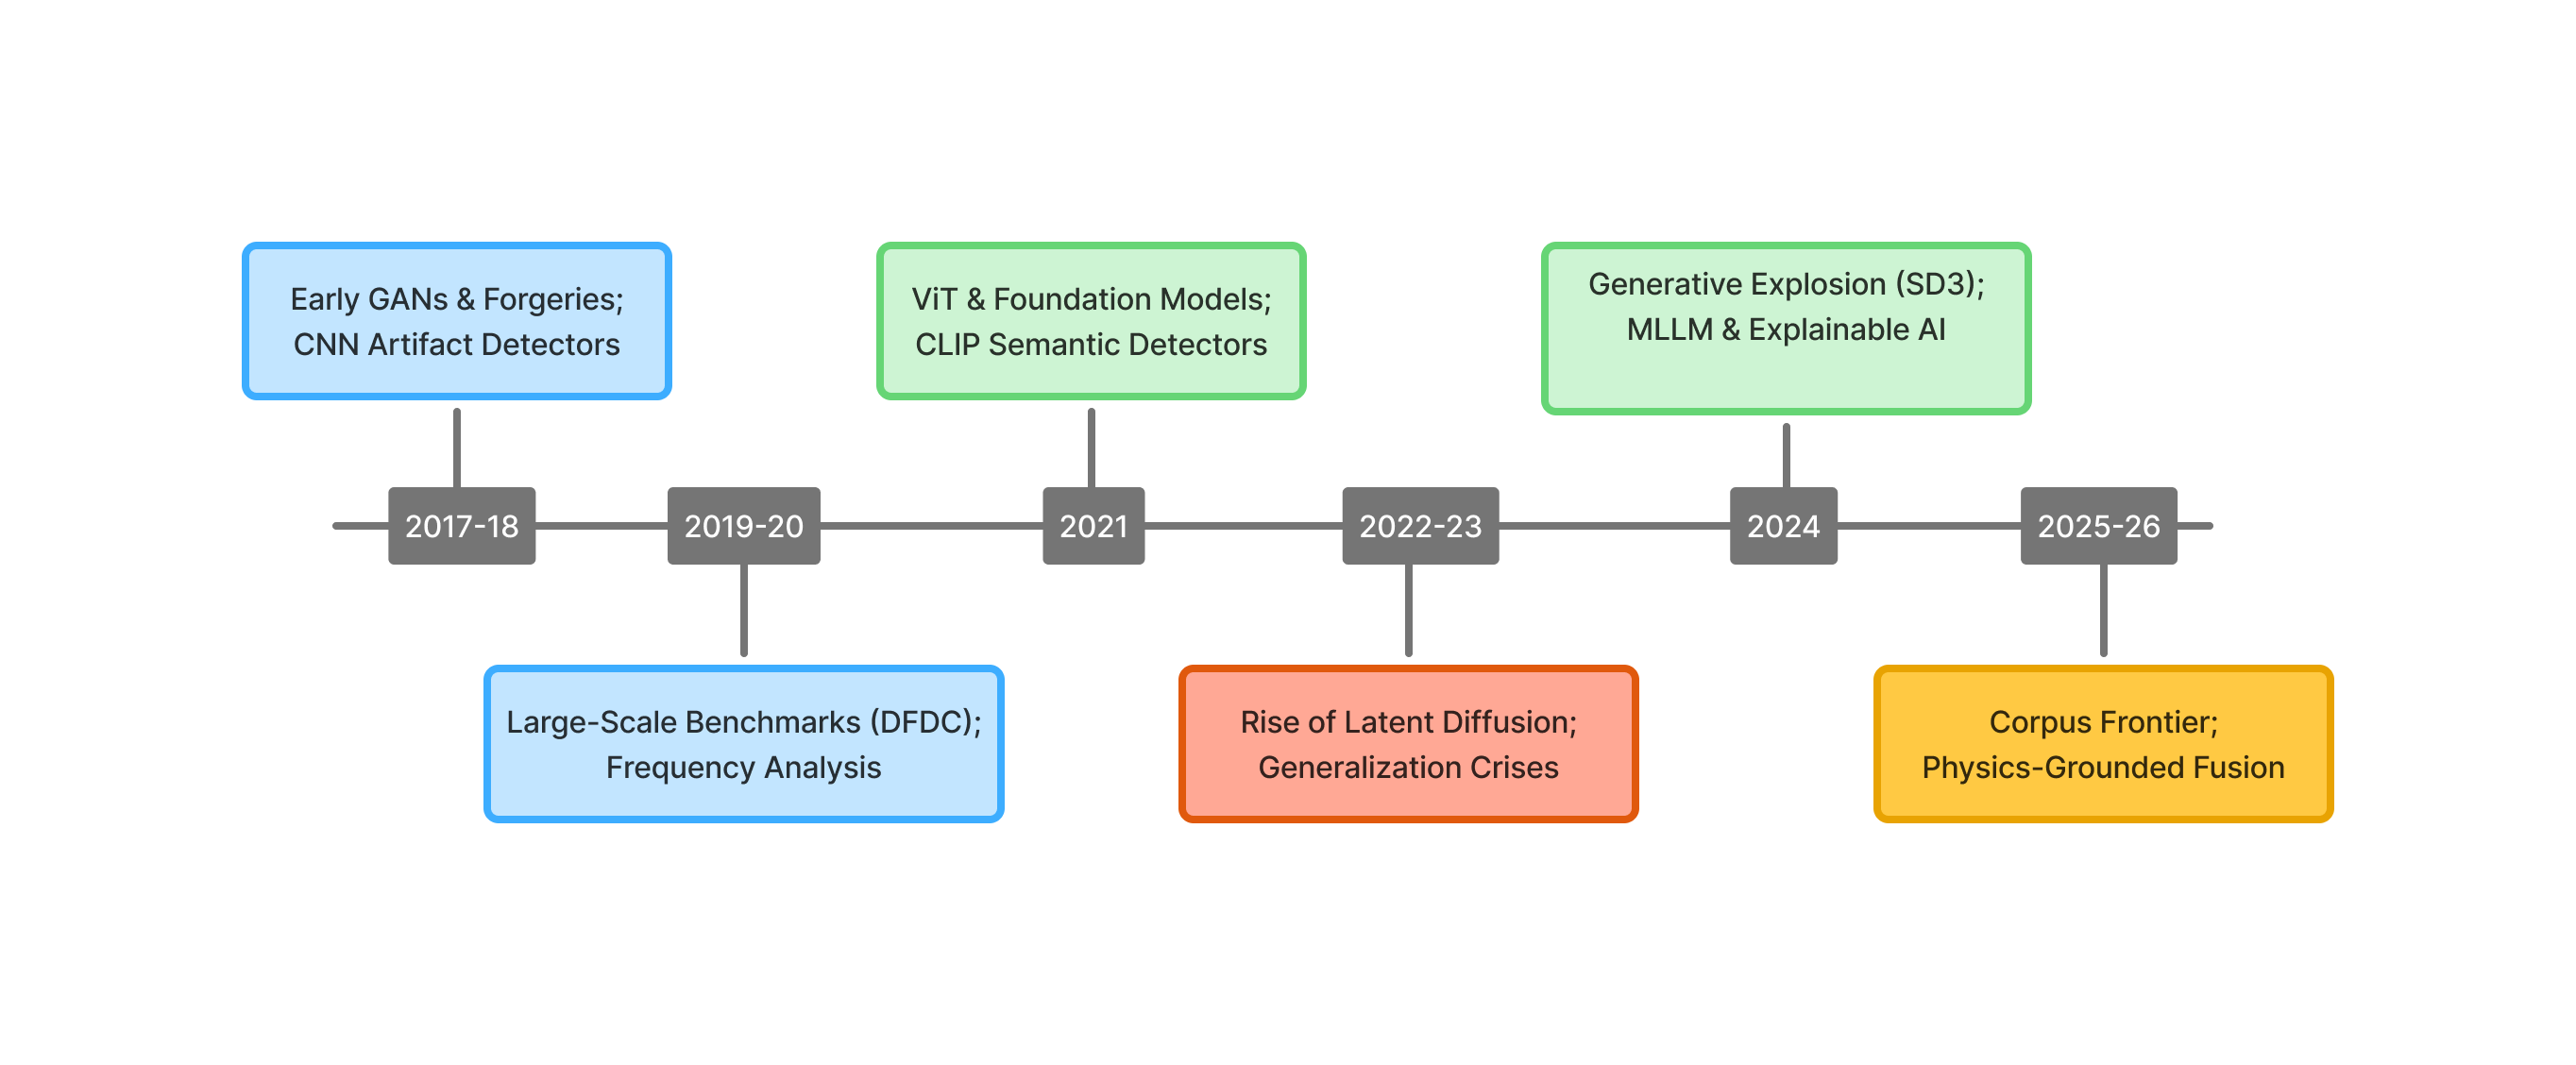
\includegraphics[width=\linewidth]{Pictures/Figure 1.png}
\caption{\textbf{Technology-evolution timeline.} The reviewed corpus occupies the right-hand frontier, where the generative explosion necessitates a shift from early artifact detectors toward physics-grounded fusion and zero-shot cross-generator evaluation.}
\label{fig:timeline}
\end{figure}
\FloatBarrier

\subsection{Objectives}
To systematically address these challenges and map the current state of the field, this paper makes the following contributions:
\begin{itemize}
\item \textbf{Methodological Taxonomy:} We organize the existing and highly fragmented technical approaches for AI-generated image and deepfake detection into a set of coherent methodological families, providing a structured lens through which disparate techniques can be compared on equal footing.

\item \textbf{Generalization Analysis:} We examine which of these families show strong empirical generalization to unseen generators and which remain highly vulnerable to performance collapse under domain shift, drawing on cross-dataset and cross-generator evaluation results reported across the literature.

\item \textbf{Physical-Consistency Evaluation:} We assess the extent to which prior work leverages physical-consistency cues, such as lighting, shadow, reflectance, geometry, depth, and anatomical plausibility, as generator-agnostic detection signals compared with traditional statistical approaches, and we consider why such cues may be more robust to the rapid architectural turnover described above.

\item \textbf{Architectural Gap Identification:} Based on the limitations observed in existing detectors, we identify a specific and evidence-based gap that motivates future development of multi-head, physics-grounded, cross-attention detection architectures capable of jointly reasoning over statistical and physical evidence.
\end{itemize}

\section{Methods}
This review follows a structured systematic-review methodology -- explicit eligibility criteria, a documented search strategy, multi-reviewer screening, and thematic narrative synthesis -- informed by established systematic-review reporting guidance \cite{Page2021}. No formal review protocol was pre-registered in an external registry (e.g., PROSPERO); this is disclosed as a limitation in Section~\ref{sec:discussion}.

\subsection{Eligibility Criteria}
\textbf{Inclusion criteria:} (i) peer-reviewed conference/journal papers, arXiv preprints, or dataset/benchmark papers whose primary contribution is a method, dataset, or empirical evaluation for detecting AI-generated or manipulated (deepfake) images, video, or audio-visual content; (ii) publications reporting a proposed detection architecture, a training/evaluation protocol, a benchmark dataset, or a systematic robustness/bias analysis of existing detectors; (iii) publications in English with an accessible abstract or full text.

\textbf{Exclusion criteria:} (i) records whose subject matter is generative modeling or a general-purpose technique with no forgery-detection application (e.g., a foundation language model or a general 3D-reconstruction method) were excluded as off-topic; (ii) secondary literature (existing surveys/systematic reviews of deepfake detection) were excluded from the primary quantitative synthesis, since this review's unit of analysis is primary technical contributions -- these secondary reviews are instead discussed narratively in Section~\ref{sec:relatedreviews} as related work; (iii) exact duplicate records (the same paper appearing twice under a preprint and a published venue, or re-entered independently during corpus compilation) were removed, retaining a single record per unique study.

\subsection{Information Sources}
Candidate records were compiled from IEEE Xplore, the ACM Digital Library, the CVF Open Access repository (CVPR/ICCV/WACV proceedings), arXiv, Semantic Scholar, SpringerLink, MDPI journals, ScienceDirect, and Hugging Face dataset listings. The corpus was last compiled and screened in July 2026.

\subsection{Search Strategy}
Search terms combined the concept of synthetic/manipulated visual media with the concept of detection, e.g.\ (``deepfake'' OR ``AI-generated image'' OR ``synthetic image'' OR ``face forgery'') AND (``detection'' OR ``forensics'' OR ``generalization'' OR ``benchmark'' OR ``cross-domain''), together with generator- and cue-specific qualifiers (``diffusion'', ``GAN'', ``CLIP'', ``physics'', ``lighting'', ``shadow'', ``geometry'', ``frequency'', ``multimodal'', ``explainable''). No date filter was applied; retrieved records span 2017--2026, reflecting both foundational forensic-vision techniques and the most recent generator-detector arms race.

\subsection{Selection Process}
The four authors jointly screened all compiled records. Records were divided among the team for an initial independent title/abstract screening pass, after which each record's inclusion/exclusion decision was cross-checked by at least one other team member against the eligibility criteria; disagreements were resolved by team discussion until consensus was reached. The same four-author team then independently assessed the remaining records at full-text level, again resolving any disagreement by discussion. A second-pass consistency check was performed collaboratively to identify duplicate records (matched by normalized title and, where available, DOI/arXiv identifier) prior to eligibility screening. No automation tools beyond spreadsheet-based deduplication were used.

\subsection{Data Collection Process and Data Items}
For each included record the following items were extracted into a structured spreadsheet: title, author(s), source link, DOI (where available), a description of the core method/approach, a summary of the paper's stated contribution, and the limitations or open gaps the paper itself reports. These items directly populate the synthesis tables in Section~\ref{sec:results}.

\subsection{Risk of Bias and Certainty Assessment}
Because the included studies are heterogeneous machine-learning method papers rather than clinical trials, a formal tool such as RoB-2 or ROBINS-I was not applicable. Instead, each study was qualitatively appraised for: (a) whether evaluation included \emph{cross-generator} or \emph{cross-dataset} testing (as opposed to only in-domain testing), (b) dataset scale and diversity, and (c) whether the paper's own stated limitations concern generalization. This appraisal is reflected in the ``Reported Gap / Limitation'' column of Tables~\ref{tab:frequency_spatial}--\ref{tab:diffusion_specific}. Publication/reporting bias was not formally quantified (e.g., no funnel plot), since the outcome of interest (cross-generator AUC) is not uniformly reported across studies in a form amenable to meta-analysis; a narrative synthesis was therefore used in place of meta-analysis, consistent with standard systematic-review guidance for methodologically heterogeneous bodies of evidence.

\subsection{Synthesis Methods}
Included studies were grouped inductively into nine thematic clusters based on their dominant technical strategy (Section~\ref{sec:results}). Within each cluster, findings are synthesized narratively, with emphasis on (i) the mechanism exploited for detection and (ii) the generalization behavior and limitations the source study itself reports. No statistical meta-analysis (e.g., pooled AUC) was performed, because studies use non-overlapping evaluation datasets, metrics, and generator sets, making quantitative pooling unreliable.

\section{Results}
\label{sec:results}

\subsection{Study Selection}
Figure~\ref{fig:prisma} presents the study identification, screening, eligibility, and inclusion flow diagram. Compilation from the sources listed in Section~II-C yielded 72 candidate records. Four records were identified as exact duplicates and removed, leaving 68 records screened by title/abstract. Four more fell out at this stage as off-topic -- a foundation language model, a text-to-image generative-modeling paper, a multi-view 3D reflectance-capture method, and a human-perception study, none of which propose or evaluate an automated forgery-detection method, even though each sits close enough to the subject matter that it warranted a second look before exclusion. The remaining 64 reports were sought and assessed at full-text level; three of those were set aside as secondary reviews or surveys rather than primary studies and are instead picked up as related work in Section~\ref{sec:relatedreviews}. What remained after this narrowing was \textbf{61 included studies}, the basis for the thematic synthesis that follows.

\begin{figure}[htbp]
\centering
\includegraphics[width=\linewidth]{Pictures/Figure 2.png}
\caption{\textbf{PRISMA study flow.} Study identification, screening, eligibility, and inclusion flow diagram.}
\label{fig:prisma}
\end{figure}
\FloatBarrier

\subsection{Study Characteristics and Thematic Synthesis}
The 61 included studies were grouped into nine thematic clusters, summarized in Table~\ref{tab:overview} and detailed in Tables~\ref{tab:frequency_spatial}--\ref{tab:diffusion_specific}. One critical observation prior to examining individual clusters is the highly uneven distribution of research focus. Low-level artifact detectors and face-specific detectors alone account for 26 of the 61 studies -- nearly half the corpus -- while physics- and scene-consistency-based detectors, the approach most directly relevant to the core architectural gap identified in this review, account for only two. This imbalance carries substantial methodological implications, which are addressed in the cross-cluster synthesis below. To better understand this landscape, Figure~\ref{fig:taxonomy} presents the architecture taxonomy of the included AI-generated image and deepfake detection studies, grouping them into four main methodological families. Furthermore, Figure~\ref{fig:distribution} shows the distribution of thematic clusters across the 61 included studies, visually emphasizing how heavily the field concentrates on low-level and face-specific detectors compared to physical modeling.

\begin{figure}[htbp]
\centering
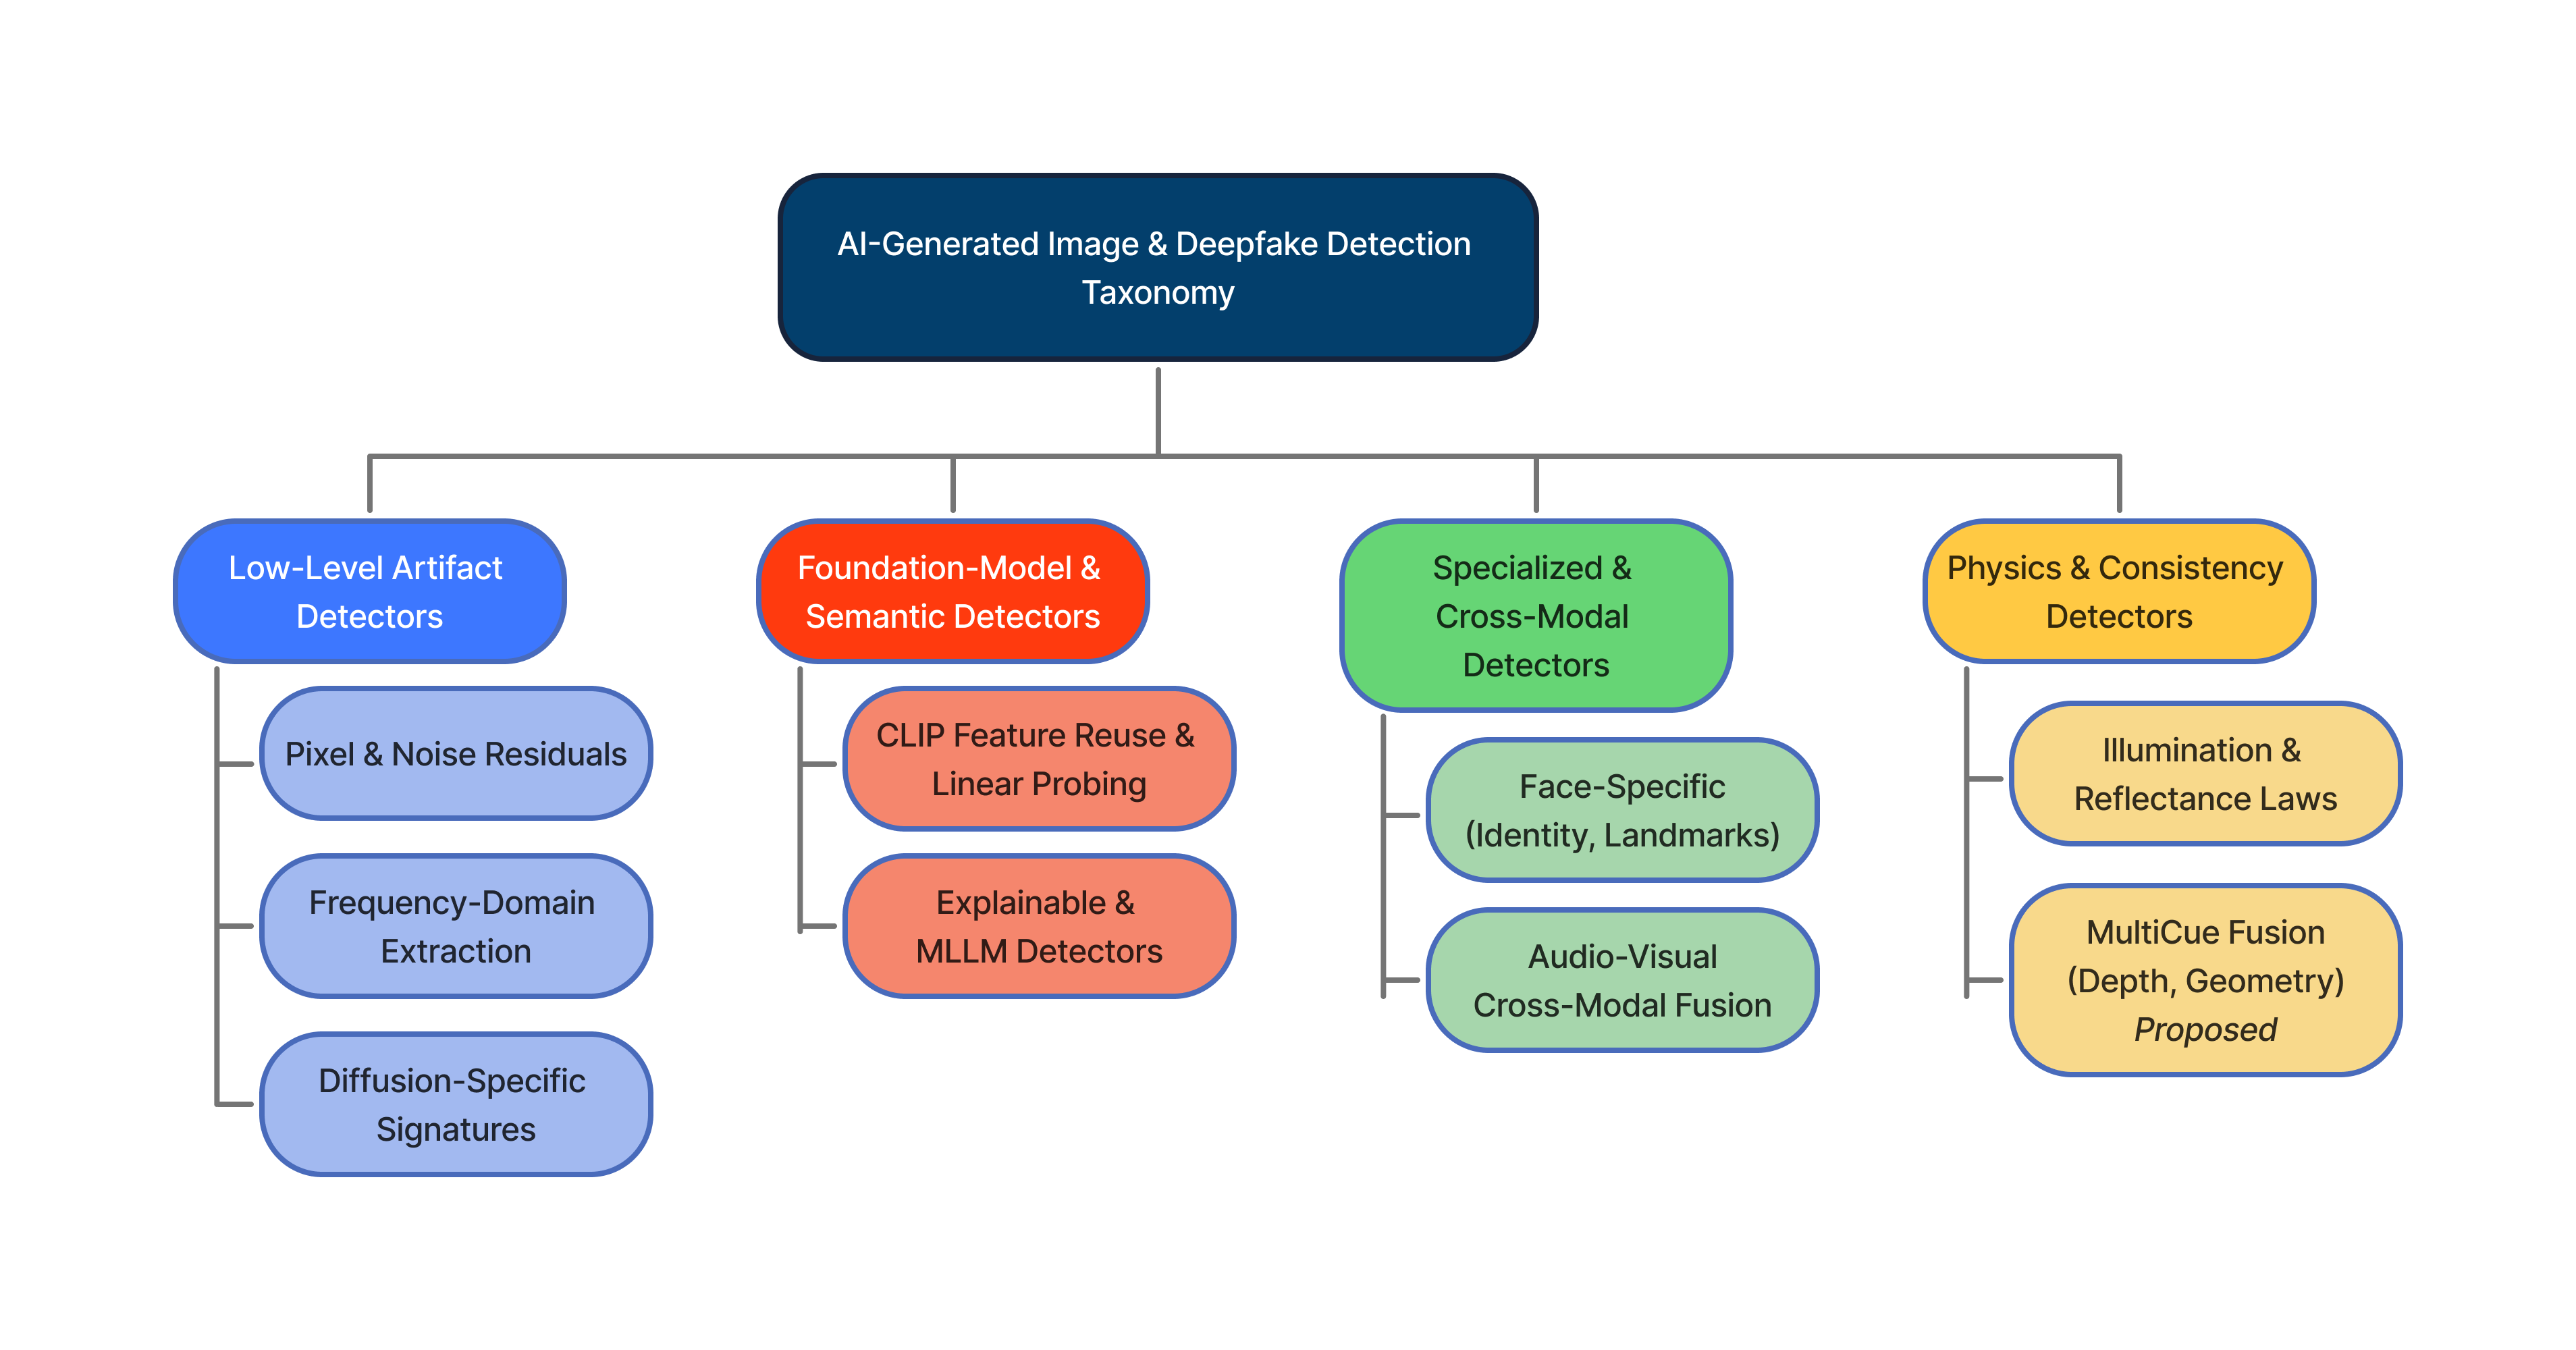
\includegraphics[width=\linewidth]{Pictures/Figure 3.png}
\caption{\textbf{Architecture taxonomy of the included AI-generated image and deepfake detection studies.} Four main methodological families are distinguished: low-level artifact detectors, foundation-model semantic detectors, specialized/cross-modal detectors, and prospective physics- and scene-consistency detectors.}
\label{fig:taxonomy}
\end{figure}
\FloatBarrier

\begin{table}[htbp]
\caption{Overview of thematic clusters among the 61 included studies}
\label{tab:overview}
\centering\footnotesize
\begin{tabularx}{\columnwidth}{@{}X c@{}}
\toprule
\textbf{Cluster} & \textbf{Studies} \\
\midrule
Low-level pixel/noise/frequency artifact detectors & 13 \\
Face-specific detectors (identity, landmark, temporal, noise) & 13 \\
Foundation-model (CLIP/vision-language) semantic detectors & 7 \\
Benchmarks and datasets & 7 \\
Robustness, bias, and generalization evaluation studies & 7 \\
Explainable and MLLM-based detectors & 6 \\
Diffusion-model-specific studies & 3 \\
Audio-visual / cross-modal fusion detectors & 3 \\
\textbf{Physics- and scene-consistency-based detectors} & \textbf{2} \\
\midrule
\textbf{Total} & \textbf{61} \\
\bottomrule
\end{tabularx}
\end{table}
\FloatBarrier

\begin{figure}[htbp]
\centering
\includegraphics[width=\linewidth]{Pictures/Figure 4.png}
\caption{\textbf{Distribution of thematic clusters across the 61 included studies.} Low-level and face-specific detectors dominate the corpus, while physics- and scene-consistency-based detectors remain markedly under-explored.}
\label{fig:distribution}
\end{figure}
\FloatBarrier

\subsection{Low-Level Pixel, Noise, and Frequency-Domain Artifact Detectors (13 studies)}
Thirteen studies -- the largest single grouping in the corpus -- build on a shared premise: generative models leave behind statistical residue, in the pixel domain, the noise domain, or the frequency spectrum, that a classifier can learn to isolate. Some train a CNN directly on RGB pixels \cite{DeepfakeImage9,AnImproved10}; others extract wavelet-domain features \cite{WaveletdrivenGeneralizable29}, isolate camera-noise residuals from a single patch \cite{ASingle32}, or model the spectral signature of real images directly \cite{AnyresolutionAigenerated33}. A recurring limitation highlighted in Table~\ref{tab:frequency_spatial} is the vulnerability of these methods to standard image transformations: compression, resizing, and blur consistently precipitate performance degradation, as these operations directly disturb the statistical fingerprints the detectors rely upon.

\begin{table}[htbp]
\caption{Included studies -- Low-Level Pixel, Noise, and Frequency-Domain Artifact Detectors}
\label{tab:frequency_spatial}
\centering\footnotesize
\begin{tabularx}{\columnwidth}{@{}p{0.10\columnwidth} X X@{}}
\toprule
\textbf{Study} & \textbf{Core Approach} & \textbf{Reported Gap / Limitation} \\
\midrule
\cite{DeepfakeImage9} & Conv2D CNN trained on large-scale OpenForensics images. & Points to future work only broadly, but its framing indicates continued need for evaluation beyond small datasets and heavy reliance on pre-trained models in prior studies. \\
\cite{AnImproved10} & Dense CNN trained on multi-source real and synthetic images. & Future work is to test variable-input networks, global pooling, and efficient image upscaling while managing the trade-off between accuracy and time latency. \\
\cite{DynamicGraph17} & Content-guided adaptive frequency extraction, multi-domain attention maps, and dynamic graph spatial-frequency fusion. & Identifies an unresolved issue in prior work: frequency features often remain spatially irrelevant and generalize poorly to increasingly realistic counterfeits. \\
\cite{DfudetectorAn18} & Feature-space restoration using a feature extractor, feature transformer, and discriminator. & Deepfake detectors still struggle when images are compressed or lose quality. Making them work well in real-world conditions is still an open challenge. \\
\cite{ArtifactFeature20} & Artifact Purification Network (APN) with frequency-band proposals. & No dedicated limitations section. Operational constraint: requires tuning the number of "frequency-band proposals" based on the difficulty of the dataset (complex datasets require more proposals). \\
\cite{ImprovingSynthetic24} & Proposes SAFE. It improves training by: Cropping instead of resizing to preserve image artifacts; Colour and rotation augmentation to reduce training bias. & SAFE still depends mainly on local pixel patterns and statistical artifacts. These features may be changed by compression, blur, resizing, or improved generators. \\
\cite{ComparativeAnalysis27} & Compares three pretrained CNN models: VGG16, VGG19, and ResNet50. It uses transfer learning to classify images as real or deepfake. & The dataset is small and the fake images come only from FaceApp. Therefore, the model may not perform well on images from unseen generators or different manipulation methods. \\
\cite{WaveletdrivenGeneralizable29} & Proposes Wavelet-CLIP. It uses a frozen CLIP ViT-L/14 model to extract image features and applies wavelet transformation to analyse both spatial and frequency information. & The method mainly focuses on facial deepfakes, so it may not work equally well on full scenes, animals, or objects. It also depends on frequency patterns, which can be affected by compression, blur, resizing, or image editing. \\
\cite{ASingle32} & Proposes SSP, which selects the simplest or least-textured patch from an image. It uses SRM filters to extract the patch's noise pattern, and ResNet-50 classifies the image as real or AI-generated. & The method depends mainly on camera-noise patterns. Compression, blur, resizing, editing, or very low-quality images can change or remove these patterns. \\
\cite{AnyresolutionAigenerated33} & Proposes SPAI, which studies images in the frequency or spectral domain. It learns the normal spectral patterns of real images and identifies AI-generated images that do not match these patterns. & The method depends mainly on spectral patterns, which can be changed by strong compression, blur, screenshots, resizing, or image editing. \\
\cite{BreakingSemantic34} & Divides each image into small patches and randomly shuffles them. This removes much of the overall scene meaning. & Shuffling patches destroys global image structure and important spatial relationships. Therefore, the method may miss errors involving lighting, shadows, perspective, depth, and object interaction. \\
\cite{MultipleContexts52} & An aggregation network that combines multiple contextual spatial scales with frequency domain transformations. & Frequency-based analysis is highly sensitive to standard video compression (like H.264 or JPEG), severely degrading real-world performance on social media. \\
\cite{CaenetGeneralized55} & A weighted ensemble architecture combining EfficientNet, Data-Efficient Image Transformer (DeiT), and ConvNeXt alongside Haar wavelet transforms. & Ensembling three distinct, heavy neural network architectures results in high computational complexity and increased inference latency. \\
\bottomrule
\end{tabularx}
\end{table}
\FloatBarrier

\subsection{Foundation-Model (CLIP/Vision-Language) Semantic-Feature Detectors (7 studies)}
An alternative strategy runs through the seven studies gathered here: rather than hand-crafting statistical detectors, they leverage large pretrained vision or vision-language models -- predominantly CLIP -- hypothesizing that internet-scale pretraining captures robust, generator-invariant semantic representations. The architectures vary: linear probing on frozen CLIP features \cite{TowardsUniversal19}, fusing several intermediate layers \cite{LeveragingRepresentations23}, decomposing the feature space with SVD \cite{OrthogonalSubspace22}, or reframing the task as image captioning with a fine-tuned vision-language model \cite{BiloraA25}. However, nearly every methodology in Table~\ref{tab:foundation_semantic} acknowledges a significant structural trade-off: the forgery signal is embedded within an opaque, high-dimensional latent space, rendering these models incapable of providing explicit, human-interpretable rationales for their classifications.

\begin{table}[htbp]
\caption{Included studies -- Foundation-Model (CLIP/Vision-Language) Semantic-Feature Detectors}
\label{tab:foundation_semantic}
\centering\footnotesize
\begin{tabularx}{\columnwidth}{@{}p{0.10\columnwidth} X X@{}}
\toprule
\textbf{Study} & \textbf{Core Approach} & \textbf{Reported Gap / Limitation} \\
\midrule
\cite{UcfUncovering16} & Disentanglement framework with multi-task learning, conditional decoding, and contrastive regularization. & Says generalization to new forgery types remains difficult, and overfitting to method-specific patterns is still insufficiently addressed. \\
\cite{TowardsUniversal19} & Nearest neighbor and linear probing on fixed CLIP-ViT feature space. & Exact visual features the pre-trained space leverages to group diverse fakes are not fully understood. Heavy Reliance on Specific Pre-training Data: The image encoder must be trained on internet-scale data (like CLIP); ImageNet fails. \\
\cite{ASanity21} & Used AIDE model, It uses two types of features: Low-level features such as noise, texture, and frequency patterns; High-level semantic features from the full image. & AIDE still struggles with highly realistic images and may classify them as real. The method also does not directly check lighting, shadows, depth, surface normals, geometry, or pose. Therefore, its results are not fully explainable. \\
\cite{OrthogonalSubspace22} & Proposes EFFORT, which uses a pretrained vision model such as CLIP. It applies Singular Value Decomposition (SVD) to divide the model's features into two separate parts. & The method learns forgery features indirectly and cannot clearly explain why an image is classified as fake. \\
\cite{LeveragingRepresentations23} & Proposes RINE. It takes features from several intermediate layers of CLIP instead of using only the final layer. & The method depends heavily on CLIP features and learns fake-image patterns indirectly. It cannot clearly explain why an image is fake. \\
\cite{BiloraA25} & Proposes Bi-LORA, which uses the BLIP-2 vision-language model with LoRA fine-tuning. It changes the detection task from normal classification into an image-captioning task. & The method depends heavily on a large pretrained vision-language model, which may require high computing resources. It learns fake-image features indirectly and cannot clearly explain why an image is classified as fake. \\
\cite{RigidA30} & Proposes RIGID, a training-free method. It adds small noise to an image and processes both the original and noisy image using a vision model such as DINOv2. It also compares their feature similarity. & The result depends on the selected vision model, noise level, and classification threshold. Highly realistic images may still be difficult to detect. \\
\bottomrule
\end{tabularx}
\end{table}
\FloatBarrier

\subsection{Physics- and Scene-Consistency-Based Detectors (2 studies)}
Only two studies in the entire corpus employ a physics-based methodology, representing the smallest cluster by a wide margin -- and, for the context of this review, arguably the most consequential one. Both operate on the intuition that light propagates according to fundamental physical laws irrespective of the generative network producing the image. Therefore, a reflectance inconsistency \cite{Light2lieDetecting2} or a Phong-model shading mismatch \cite{DigitalImage42} should theoretically remain robust against unseen generators. In practice, however, Table~\ref{tab:physics_based} highlights that both studies are limited to single-cue analysis, require manual patch selection, and fail on complex scenes where multiple objects share parallel lighting parameters. This combination—promising in theory, yet limited in practical application—is examined further in Section~\ref{sec:discussion}.

\begin{table}[htbp]
\caption{Included studies -- Physics- and Scene-Consistency-Based Detectors}
\label{tab:physics_based}
\centering\footnotesize
\begin{tabularx}{\columnwidth}{@{}p{0.10\columnwidth} X X@{}}
\toprule
\textbf{Study} & \textbf{Core Approach} & \textbf{Reported Gap / Limitation} \\
\midrule
\cite{Light2lieDetecting2} & Physics-based deepfake detection using physical reflectance laws. & Frames the remaining gap as poor generalization to unseen generators, weak physical grounding in existing methods, vulnerability to adaptive attacks, and limited interpretability. \\
\cite{DigitalImage42} & Phong reflection model approach to analyze scene inconsistencies in the direction of light. & Requires manual object patch selection. Fails if spliced images share identical lighting angles. Incompatible with image fusion-based forgeries. Validated in controlled environments; unknown parameters limit effectiveness. \\
\bottomrule
\end{tabularx}
\end{table}
\FloatBarrier

\subsection{Explainable and Multimodal-LLM-Based Detectors (6 studies)}
To address the interpretability deficit observed in the foundation-model cluster, six studies prioritize explainability. Some attribute an image to its likely source model and analyze the prompting conditions \cite{DefakeDetection12}; others generate comprehensive, human-readable rationales using large multimodal models (LMMs) \cite{AigiholmesTowards13,SpotThe58}, or trace structural inconsistencies across diffusion timesteps \cite{ExplainableSynthetic59}. The computational cost of this capability is evident in Table~\ref{tab:explainable_mllm}: generating a linguistic rationale via an LMM incurs substantial computational overhead compared to a standard forward pass through a traditional classifier, complicating deployment in high-throughput environments.

\begin{table}[htbp]
\caption{Included studies -- Explainable and Multimodal-LLM-Based Detectors}
\label{tab:explainable_mllm}
\centering\footnotesize
\begin{tabularx}{\columnwidth}{@{}p{0.10\columnwidth} X X@{}}
\toprule
\textbf{Study} & \textbf{Core Approach} & \textbf{Reported Gap / Limitation} \\
\midrule
\cite{DefakeDetection12} & Machine-learning fake-image detector with source-model attribution and prompt analysis across four text-to-image models. & The open gap is robustness to rapidly evolving text-to-image models and to prompt conditions that produce more authentic images, especially person-related or medium-length prompts. \\
\cite{AigiholmesTowards13} & Three-stage Holmes Pipeline with visual expert pre-training, supervised fine-tuning, direct preference optimization, and collaborative decoding. & Explicitly says prior AIGI detection still lacks human-verifiable explanations and does not generalize well to the latest generation technology. \\
\cite{ZerofakeZeroshot47} & A zero-shot, training-free framework utilising perturbation-based DDIM inversion and reconstruction guided by adversary prompts. & High computational time and hardware overhead during the inference phase. On an NVIDIA DGX-A100, the DDIM inversion and reconstruction process takes 30.2 seconds per image. \\
\cite{ExplainableAi48} & A two-stage pipeline: (1) deepfake detection using ResNet-50, Inception V3, and VGG-16 classifiers trained on the Celeb-DF dataset. & The model's interpretability is constrained by the narrow range of facial concepts present in the deepfake face dictionary. \\
\cite{SpotThe58} & Prompting and feature extraction using Large Multimodal Models (LMMs) for artifact localization and explanation. & The massive parameter size of LMMs causes significant computational overhead, making real-time or high-throughput detection impractical. \\
\cite{ExplainableSynthetic59} & Analyzing noise patterns and structural inversions across multiple timesteps of the diffusion generation process. & The methodology is strictly tied to diffusion architectures and is ineffective against older GAN-based or manual manipulation techniques. \\
\bottomrule
\end{tabularx}
\end{table}
\FloatBarrier

\subsection{Face-Specific Deepfake Detectors (Identity, Landmark, Temporal, Noise) (13 studies)}
Thirteen studies -- matching the low-level cluster in volume -- restrict their scope strictly to human faces, targeting identity swaps, expression transfers, and temporal anomalies across video frames \cite{ContrastivePseudo1,DynamicSpatialtemporal50,TowardsGeneralizable49}. Several explicitly formulate the detection task as a domain generalization problem, attempting to isolate forgery-relevant features from dataset-specific backgrounds \cite{CrossdfImproving44,GmdfGeneralized37}. While the results in Table~\ref{tab:face_specific} demonstrate strong intra-domain performance, a recurring caveat emerges: because these architectures and evaluation protocols are highly specialized to facial morphology, their efficacy on full-scene synthetic generation or non-facial manipulation remains speculative and largely untested.

\begin{table}[htbp]
\caption{Included studies -- Face-Specific Deepfake Detectors (Identity, Landmark, Temporal, Noise)}
\label{tab:face_specific}
\centering\footnotesize
\begin{tabularx}{\columnwidth}{@{}p{0.10\columnwidth} X X@{}}
\toprule
\textbf{Study} & \textbf{Core Approach} & \textbf{Reported Gap / Limitation} \\
\midrule
\cite{ContrastivePseudo1} & Contrastive Pseudo Learning with Global-Local Voting, confidence-based soft pseudo-labels, and multi-stage iterative learning for open-world attribution. & Says identity swapping, expression transfer, and forgery traces in unknown open-world unlabeled faces remain under-explored, indicating future work on broader attack coverage and open-world interpretability. \\
\cite{NoiseBased5} & Noise-based detector using enhanced RIDNet and Multi-Head Relative-Interaction between face and background. & Leaves open the challenge that increasingly realistic deepfakes show few visible differences, so methods that depend on stronger and more invariant forensic traces are still needed. \\
\cite{AHybrid26} & Uses a hybrid CNN-LSTM model with transfer learning. The CNN extracts visual features from face images, while the LSTM learns relationships between these features. & The method mainly focuses on facial deepfakes and does not test images from completely unseen generators. Its high results may not represent real-world generalization. \\
\cite{GmdfGeneralized37} & Proposes GM-DF, which trains one model using multiple deepfake datasets. It uses expert branches to learn dataset-specific features and CLIP to learn common forgery features. & The method mainly focuses on facial deepfakes, so it may not work equally well on full scenes, animals, or objects. \\
\cite{FinegrainedOpenset38} & Uses labelled deepfake images from a source dataset and unlabelled images from a target dataset. It groups the target images using adaptive clustering and gives them pseudo-labels. & The method requires access to unlabelled images from the target domain, so it is not fully zero-shot. \\
\cite{FaceForgery39} & Combines spatial features from the original face image with noise features that reveal hidden forgery traces. & The method mainly focuses on facial deepfakes, so it may not work equally well on animals, objects, or complete AI-generated scenes. \\
\cite{OpensetDeepfake40} & Proposes OSDFD, which uses a pretrained Vision Transformer. It adds lightweight LoRA and adapter modules to learn global and local forgery features without training the whole model. & The method mainly focuses on facial deepfakes, so it may not work equally well on animals, objects, or full AI-generated scenes. \\
\cite{CrossdfImproving44} & Deep Information Decomposition (DID) framework that formulates cross-dataset deepfake detection as a domain generalization problem. & All hyperparameters in the loss function require manual tuning through extensive experimental trials, which is inefficient and suboptimal. The domain classification module depends on explicit domain-specific metadata. \\
\cite{TowardsGeneralizable49} & The LGMamba network, which parallelly combines global long-range modelling (via a VMamba visual State-Space backbone) with local feature extraction. & Fails to model temporal dependencies. Because it is strictly designed for frame-level spatial analysis, it is less effective on video datasets (like DFD) where manipulation operations involve frame interpolation or dropping. \\
\cite{DynamicSpatialtemporal50} & The Dynamic Spatial-Temporal Network (DST-Net), integrating: (1) Short-term Temporal Modality Extraction (STME) to compute gradient differences between consecutive frames. & The dynamic attention mechanisms and multi-scale temporal aggregation increase the overall computational cost, which may limit deployment in real-time or resource-constrained settings. \\
\cite{DeepfakeDetection57} & Supervised fine-tuning of a standard Convolutional Neural Network for binary (real/fake) spatial classification. & Pure CNNs struggle heavily with cross-domain generalization and often fail completely on unseen modern diffusion models. \\
\cite{DeepshieldFortifying61} & Combines Local Patch Guidance (LPG) and Global Forgery Diversification (GFD) using a fine-tuned CLIP-ViT backbone with a 3D spatiotemporal adapter. & The reliance on temporal 3D convolutions increases computational overhead, complicating deployment for live streaming applications. \\
\cite{DelocateDetection63} & A two-stage framework utilizing a masked autoencoder trained only on real faces for consistency learning, followed by a localization module. & The initial recovery phase depends entirely on high-quality, completely untampered real faces, making the training sensitive to noisy data. \\
\bottomrule
\end{tabularx}
\end{table}
\FloatBarrier

\subsection{Benchmarks and Datasets (7 studies)}
Seven of the included studies function as the foundational infrastructure for generalization testing rather than standalone detectors. This includes standardized benchmarks spanning multiple methods and datasets \cite{DeepfakebenchA4}, massive in-the-wild image compilations \cite{TowardsRealworld56,WildfakeA66}, and continuously updated frameworks interfacing directly with commercial APIs \cite{AigenbenchA72}. A persistent limitation highlighted in Table~\ref{tab:benchmark_dataset} is temporal decay: evaluation benchmarks become outdated rapidly as generative architectures iterate, an issue frequently acknowledged by the dataset authors themselves \cite{TowardsRealworld56,Deepfakeeval2024A64}.

\begin{table}[htbp]
\caption{Included studies -- Benchmarks and Datasets}
\label{tab:benchmark_dataset}
\centering\footnotesize
\begin{tabularx}{\columnwidth}{@{}p{0.10\columnwidth} X X@{}}
\toprule
\textbf{Study} & \textbf{Core Approach} & \textbf{Reported Gap / Limitation} \\
\midrule
\cite{DffmdA3} & Inception-ResNet-v2 with preprocessing, residual connection, feature extraction, and batch normalization on a face-mask dataset. & The attached paper explicitly reports a lack of masked-face video resources and calls for more deep learning experiments for masked deepfake detection. \\
\cite{DeepfakebenchA4} & Unified benchmark with standardized data management, implementations, and evaluation protocols across 15 methods and 9 datasets. & The remaining need is field-wide adoption and extension of uniform preprocessing, settings, and metrics, because inconsistent pipelines still produce unfair or misleading comparisons. \\
\cite{TowardsRealworld56} & Massive data curation and benchmark testing using diverse, "in-the-wild" manipulations. & Static datasets, no matter how diverse, rapidly lose relevance as newer, superior generative AI architectures are released. \\
\cite{ImaginetA60} & Creation of a multi-content, zero-shot evaluation benchmark spanning diverse semantic classes. & Focuses purely on benchmarking existing models rather than offering a new, functional detection mechanism. \\
\cite{Deepfakeeval2024A64} & Multi-modal empirical evaluation of state-of-the-art detectors against circulating, real-world 2024 media content. & Specifically bounded to 2024 generative capabilities, requiring constant future updates to remain a relevant metric. \\
\cite{WildfakeA66} & Large-scale dataset compilation focused on highly challenging, complex, and unconstrained AI-generated images. & Like many large datasets, it lacks fine-grained annotations regarding the specific generative parameters or prompts used to create the images. \\
\cite{AigenbenchA72} & An ongoing, continuously updated evaluation framework integrating outputs directly from new generative APIs. & Requires immense constant maintenance, persistent API access, and heavy computational resources to keep the benchmark up to date. \\
\bottomrule
\end{tabularx}
\end{table}
\FloatBarrier

\subsection{Robustness, Bias, and Generalization Evaluation Studies (7 studies)}
Whereas the benchmark cluster constructs new evaluation sets, these seven studies instead evaluate existing detectors to expose their vulnerabilities. This literature documents systemic biases baked into training corpora—such as JPEG compression artifacts or resolution disparities between real and synthetic classes \cite{FakeOr35}—and evaluates models against customized adversarial attacks or content-preserving perturbations \cite{AnAnalysis36,AdversarialRobustness65,ComprehensiveEvaluation46}. The overarching finding in Table~\ref{tab:robustness_bias} reveals a critical vulnerability in current detection methodologies: a detector's reported accuracy can often be attributed to dataset biases rather than genuine forgery detection. This confound underscores the necessity for the rigorous evaluation protocols discussed in Section~\ref{sec:discussion}.

\begin{table}[htbp]
\caption{Included studies -- Robustness, Bias, and Generalization Evaluation Studies}
\label{tab:robustness_bias}
\centering\footnotesize
\begin{tabularx}{\columnwidth}{@{}p{0.10\columnwidth} X X@{}}
\toprule
\textbf{Study} & \textbf{Core Approach} & \textbf{Reported Gap / Limitation} \\
\midrule
\cite{QualityagnosticDeepfake8} & Quality-agnostic single-model detector using HSIC-based collaborative learning and adversarial weight perturbation. & Low-quality and mixed-quality deepfake detection remains a grave challenge, and multi-model quality-specific setups are still computationally costly and impractical for deployment. \\
\cite{ABiasfree31} & Proposes B-Free. It creates fake images from real COCO images using Stable Diffusion 2.1, so the real and fake images have similar content. & The training images are mainly generated using Stable Diffusion 2.1, so the model may fail on future generators that use a very different generation process. It can also be affected by adversarial attacks. \\
\cite{FakeOr35} & Studies JPEG compression and image-size bias in AI-generated image datasets. It creates a corrected version of GenImage by making the real and generated images more similar in compression and resolution. & Mainly studies dataset bias and does not propose a new detection architecture. Its experiments focus mostly on GenImage and two detector models, so other datasets may contain different biases. \\
\cite{AnAnalysis36} & Evaluates eight deepfake detectors using images from 16 customized Stable Diffusion models. It also tests an attack that changes image content using vision foundation models without adding visible noise. & Mainly uses customized Stable Diffusion models, so the results may not cover every GAN or modern image generator. \\
\cite{ComprehensiveEvaluation46} & Attaches custom classification heads to three pre-trained convolutional neural networks (CNNs): XCeption (depthwise separable convolutions), ResNet (ResNet-50 and ResNet-101 ensemble predictions), and VGG16. & All models suffer from pervasive vulnerability to adversarial attacks, with accuracy dropping significantly under mild FGSM perturbations. \\
\cite{PreservingFairness62} & Fairness-aware regularization techniques applied across varying demographic training subsets. & Implementing strict fairness constraints often results in a mathematical trade-off, slightly lowering overall absolute detection accuracy. \\
\cite{AdversarialRobustness65} & Applying gradient-based adversarial perturbations and common image degradations to test model resilience. & Acts purely as a vulnerability assessment rather than providing a standalone, robust defensive architecture to solve the problem. \\
\bottomrule
\end{tabularx}
\end{table}
\FloatBarrier

\subsection{Audio-Visual and Cross-Modal Fusion Detectors (3 studies)}
Three studies expand the detection perimeter beyond single-image analysis, fusing audio and visual streams \cite{ARobust11,ContextualCrossmodal68} or combining spatial and frequency pathways within the visual modality itself \cite{AMultimodal69}. This cross-modal perspective leverages incongruencies unavailable in static media, such as lip-sync mismatches; however, as noted in Table~\ref{tab:audiovisual_multimodal}, these frameworks are inherently inapplicable to single static images, which constitute the primary focus of this review.

\begin{table}[htbp]
\caption{Included studies -- Audio-Visual and Cross-Modal Fusion Detectors}
\label{tab:audiovisual_multimodal}
\centering\footnotesize
\begin{tabularx}{\columnwidth}{@{}p{0.10\columnwidth} X X@{}}
\toprule
\textbf{Study} & \textbf{Core Approach} & \textbf{Reported Gap / Limitation} \\
\midrule
\cite{ARobust11} & Audio-visual temporal feature extraction with time-aware neural networks and multimodal fusion trained on disjoint monomodal datasets. & Explicitly proposes future work on new fusion methods, especially informed fusion that weights modalities by relevance; the broader limitation is the scarcity of multimodal training datasets. \\
\cite{ContextualCrossmodal68} & Cross-modal attention networks that analyze the synchronization between audio tracks and visual lip movements. & Completely ineffective on image-only deepfakes, silent videos, or heavily dubbed media. \\
\cite{AMultimodal69} & Multi-stream feature extraction architecture combining spatial (RGB) and frequency data pathways. & Requires processing multiple dense data streams simultaneously, leading to higher resource consumption during inference. \\
\bottomrule
\end{tabularx}
\end{table}
\FloatBarrier

\subsection{Diffusion-Model-Specific Detection Studies (3 studies)}
The final three studies exhibit a narrow focus on specific generator families rather than cross-modal fusion. This includes diffusion-specific benchmarks incorporating degraded-image testing \cite{RobustnessAnd7}, profiling spatial and frequency signatures intrinsic to latent diffusion sampling \cite{DiffusionDeepfake70}, and baseline evaluations of CNNs against early diffusion outputs \cite{TowardsThe71}. Table~\ref{tab:diffusion_specific} indicates that this deep specialization severely limits backward compatibility with GAN-based manipulations, and explicitly risks rapid obsolescence as newer architectures like Stable Diffusion 3 and Flux.1 redefine the artifact landscape.

\begin{table}[htbp]
\caption{Included studies -- Diffusion-Model-Specific Detection Studies}
\label{tab:diffusion_specific}
\centering\footnotesize
\begin{tabularx}{\columnwidth}{@{}p{0.10\columnwidth} X X@{}}
\toprule
\textbf{Study} & \textbf{Core Approach} & \textbf{Reported Gap / Limitation} \\
\midrule
\cite{RobustnessAnd7} & Diffusion-based DFF dataset with cross-generator and degraded-image evaluation protocols. & Detector performance still varies across generative methods and image degradations, so more universally robust detectors and finer analysis of perturbation effects remain open. \\
\cite{DiffusionDeepfake70} & Profiling and detecting the specific spatial and frequency signatures inherent to latent diffusion models. & Focuses almost exclusively on diffusion-based models, limiting its generalization capability against legacy manipulation techniques like FaceSwap. \\
\cite{TowardsThe71} & Evaluating standard CNN and Vision Transformer (ViT) classification baselines against early diffusion model outputs. & Conducted on older (2022 era) diffusion models, making its specific empirical findings somewhat outdated for modern generators like SD3 or Flux. \\
\bottomrule
\end{tabularx}
\end{table}
\FloatBarrier

\subsection{Cross-Cluster Synthesis}

\subsubsection{Low-level artifact learners generalize poorly}
The largest cluster (13/61 studies) consists of detectors that classify images using pixel-, noise-, or frequency-domain statistics -- GAN checkerboard patterns, sensor-noise residuals, or spectral signatures extracted via wavelets or Fourier analysis \cite{ArtifactFeature20,AnyresolutionAigenerated33,MultipleContexts52,CaenetGeneralized55,WaveletdrivenGeneralizable29,BreakingSemantic34}. These methods routinely report strong in-domain accuracy but explicitly flag degradation under compression, resizing, or when tested against generator families absent from training. This corroborates a central premise of the field: fingerprint-style detectors do not transfer across generator boundaries. These detectors optimize for the residue of a specific sampling pipeline; consequently, when the underlying architecture or training corpus changes, the specific statistical signals evaporate.

\subsubsection{Foundation-model semantic features generalize better, but remain indirect}
Seven studies exploit large pretrained vision(-language) backbones, chiefly CLIP, either via linear probing \cite{TowardsUniversal19}, intermediate-layer fusion \cite{LeveragingRepresentations23}, orthogonal/SVD feature decomposition \cite{OrthogonalSubspace22}, or vision-language captioning reframing \cite{BiloraA25}. These approaches consistently report markedly better cross-generator AUC than low-level detectors, supporting the hypothesis that broad, internet-scale pretraining captures more generator-invariant structure than architecture-specific noise statistics. However, every study self-reports a fundamental limitation: the detector learns forgery cues \emph{indirectly}, through an opaque embedding, and therefore cannot explain \emph{why} an image is classified as synthetic, posing significant challenges for forensic interpretability.

\subsubsection{Physics-based detection is the least explored and most under-resourced cluster}
Only two of the 61 included studies pursue physical-consistency modeling directly \cite{Light2lieDetecting2,DigitalImage42}. Both report that physics-based scene analysis generalizes across generator architectures \emph{by construction}, because lighting, shadow, and reflectance laws hold regardless of which network produced the pixels. However, both rely on shallow, single-cue implementations (a single reflectance law, or a Phong-model shading check) that require manual patch selection and fail on complex or fused scenes. Related but non-detection physics literature -- multi-view geometry/reflectance capture \cite{Deep3DCaptureExcluded} and human-perception studies of physical implausibility in manipulated photographs \cite{CanPeopleExcluded} -- corroborates that physical implausibility is a robust, human-relevant detection signal. Together, this indicates a substantial gap: physical cues offer theoretical robustness to domain shift, yet the literature has rarely advanced beyond single-cue proofs of concept.

\subsubsection{Face-specific and explainable/MLLM clusters address complementary needs}
The face-specific cluster targets identity-swap and expression-transfer artifacts using landmark-guided convolution \cite{TowardsGeneralizable49} or spatiotemporal inconsistency modeling \cite{DynamicSpatialtemporal50}, but remains architecturally constrained to human faces. Conversely, the explainable/MLLM cluster prioritizes interpretability, utilizing large multimodal models to narrate detected artifacts \cite{AigiholmesTowards13,SpotThe58}, though at significant computational expense and without natively structuring reasoning around geometric or physical constraints. A highly promising research avenue involves synthesizing these objectives: developing a framework that is lightweight, applicable to full scenes, and inherently interpretable.

\subsubsection{Benchmarks confirm the generalization gap empirically}
The seven benchmark/dataset studies are foundational for cross-generator evaluation. Several explicitly report that detectors trained on older GAN or early-diffusion corpora collapse when evaluated against 2024--2026 generators such as Flux.1 and SD3 \cite{Deepfakeeval2024A64, AigenbenchA72}, directly motivating the necessity for disjoint training (Domain A) and testing (Domain B) distributions in future architectural evaluations. These testbeds confirm that genuine robustness can only be verified via systematic out-of-distribution testing.

\subsubsection{Robustness/bias studies reveal confounds beyond generator identity}
Seven studies document that reported accuracy metrics are frequently inflated by dataset construction artifacts—such as resolution disparities or JPEG compression biases between real and synthetic classes \cite{FakeOr35}—or remain highly susceptible to basic adversarial perturbations \cite{AdversarialRobustness65}. This has a direct methodological implication for future detection frameworks: any zero-shot cross-generator evaluation must rigorously control for compression and resolution confounds, alongside generator identity, to validate true generalization.

\subsection{Related Reviews Excluded from Primary Synthesis}
\label{sec:relatedreviews}
Three secondary review articles were identified and excluded from the quantitative synthesis (per Section II-A) but provide vital context. A systematic review of deep-learning-based detection across diverse media formats reported that inconsistently described literature impeded reliable cross-method comparison \cite{HeidariReviewExcluded}. A review of fusion-based methods highlighted cross-dataset generalization, interpretability, and lightweight deployment as defining the future research agenda \cite{GuptaReviewExcluded}. A recent survey confirmed the field's shift toward generalizable, automated evaluation frameworks \cite{SunilSurveyExcluded}. All three converge independently on the conclusion that generalization to unseen generators, rather than raw in-domain accuracy, remains the primary bottleneck for forensic verification.

\section{Discussion}
\label{sec:discussion}

Before interpreting the specific findings across clusters, it is necessary to view the limitations of the field holistically. Figure~\ref{fig:gapmap} presents a research-gap map over representative studies and recurrent gap dimensions. The near-uniform columns for cross-generator generalization and physical cues indicate systemic, field-wide gaps.

\begin{figure}[htbp]
\centering
\includegraphics[width=\linewidth]{Pictures/Figure 5.png}
\caption{\textbf{Research-gap map over representative studies and recurrent gap dimensions.} Cells encode whether each gap is addressed, partially addressed, or present. The near-uniform columns for cross-generator generalization and physical cues indicate systemic, field-wide gaps.}
\label{fig:gapmap}
\end{figure}
\FloatBarrier

\subsection{Interpretation}
Synthesizing across all nine clusters, three primary findings emerge. First, detection strategies form a functional generalization hierarchy: low-level statistical detectors generalize poorly, pretrained semantic detectors generalize moderately well but remain opaque, and physics-based strategies generalize effectively \emph{in principle} but remain under-developed in practice. Second, physical-consistency modeling is empirically under-explored (2/61 studies) relative to its theoretical promise, with no included studies successfully integrating multiple physical cues (lighting, depth, surface normals, and pose) within a unified, generator-agnostic architecture. Third, this gap highlights the need for cross-attention, multi-head physical-signal fusion architectures. Such candidate frameworks could generalize the single-cue physics detectors identified in Section III-B-iii into a multi-cue system, while retaining the interpretability that foundation-model and MLLM-based detectors lack, by explicitly outputting localized physical mismatches.

\subsection{Limitations of the Evidence}
Several included studies rely on modest, single-domain datasets (e.g., FaceApp-only subsets), limiting the generalizability of their empirical claims. Furthermore, reported metrics (AUC, accuracy, EER) are not uniformly defined or measured on comparable held-out test sets across the literature, precluding robust statistical meta-analysis and necessitating the narrative synthesis presented here.

\subsection{Limitations of the Review Process}
This review was conducted by a four-author team utilizing consensus-based screening, which diverges from fully blinded dual-independent review protocols. Additionally, no external protocol registration (e.g., PROSPERO) was performed. The search strategy did not exhaustively query all scientific indices (e.g., Scopus, Web of Science), and grey literature outside of arXiv preprints was not systematically targeted. While the multi-author screening mitigates individual selection bias, shared conceptual boundaries during search-term formulation represent a potential limitation.

\subsection{Implications for Practice and Future Research}
The synthesis directly motivates a candidate research direction in which (i) a multi-head architecture independently estimates illumination/shadow dynamics, surface normals, monocular depth, and geometric pose from an input image; (ii) a cross-attention fusion module identifies \emph{inconsistencies between} these physical modalities rather than implicitly memorizing network-specific fingerprints; and (iii) the model is trained exclusively on legacy generators (Domain A: FFHQ, FaceForensics++, GenImage) and evaluated strictly zero-shot against contemporary generation engines (Domain B: GenImage++, Defactify, 2024–2026 models). This protocol aligns precisely with the stringent evaluation logic demonstrated by the benchmark cluster (Section III-B-v). To operationalize this agenda, Figure~\ref{fig:roadmap} sequences the prospective research directions into short-, medium-, and long-term phases, charting a pathway toward comprehensive physical consistency verification.

\begin{figure}[htbp]
\centering
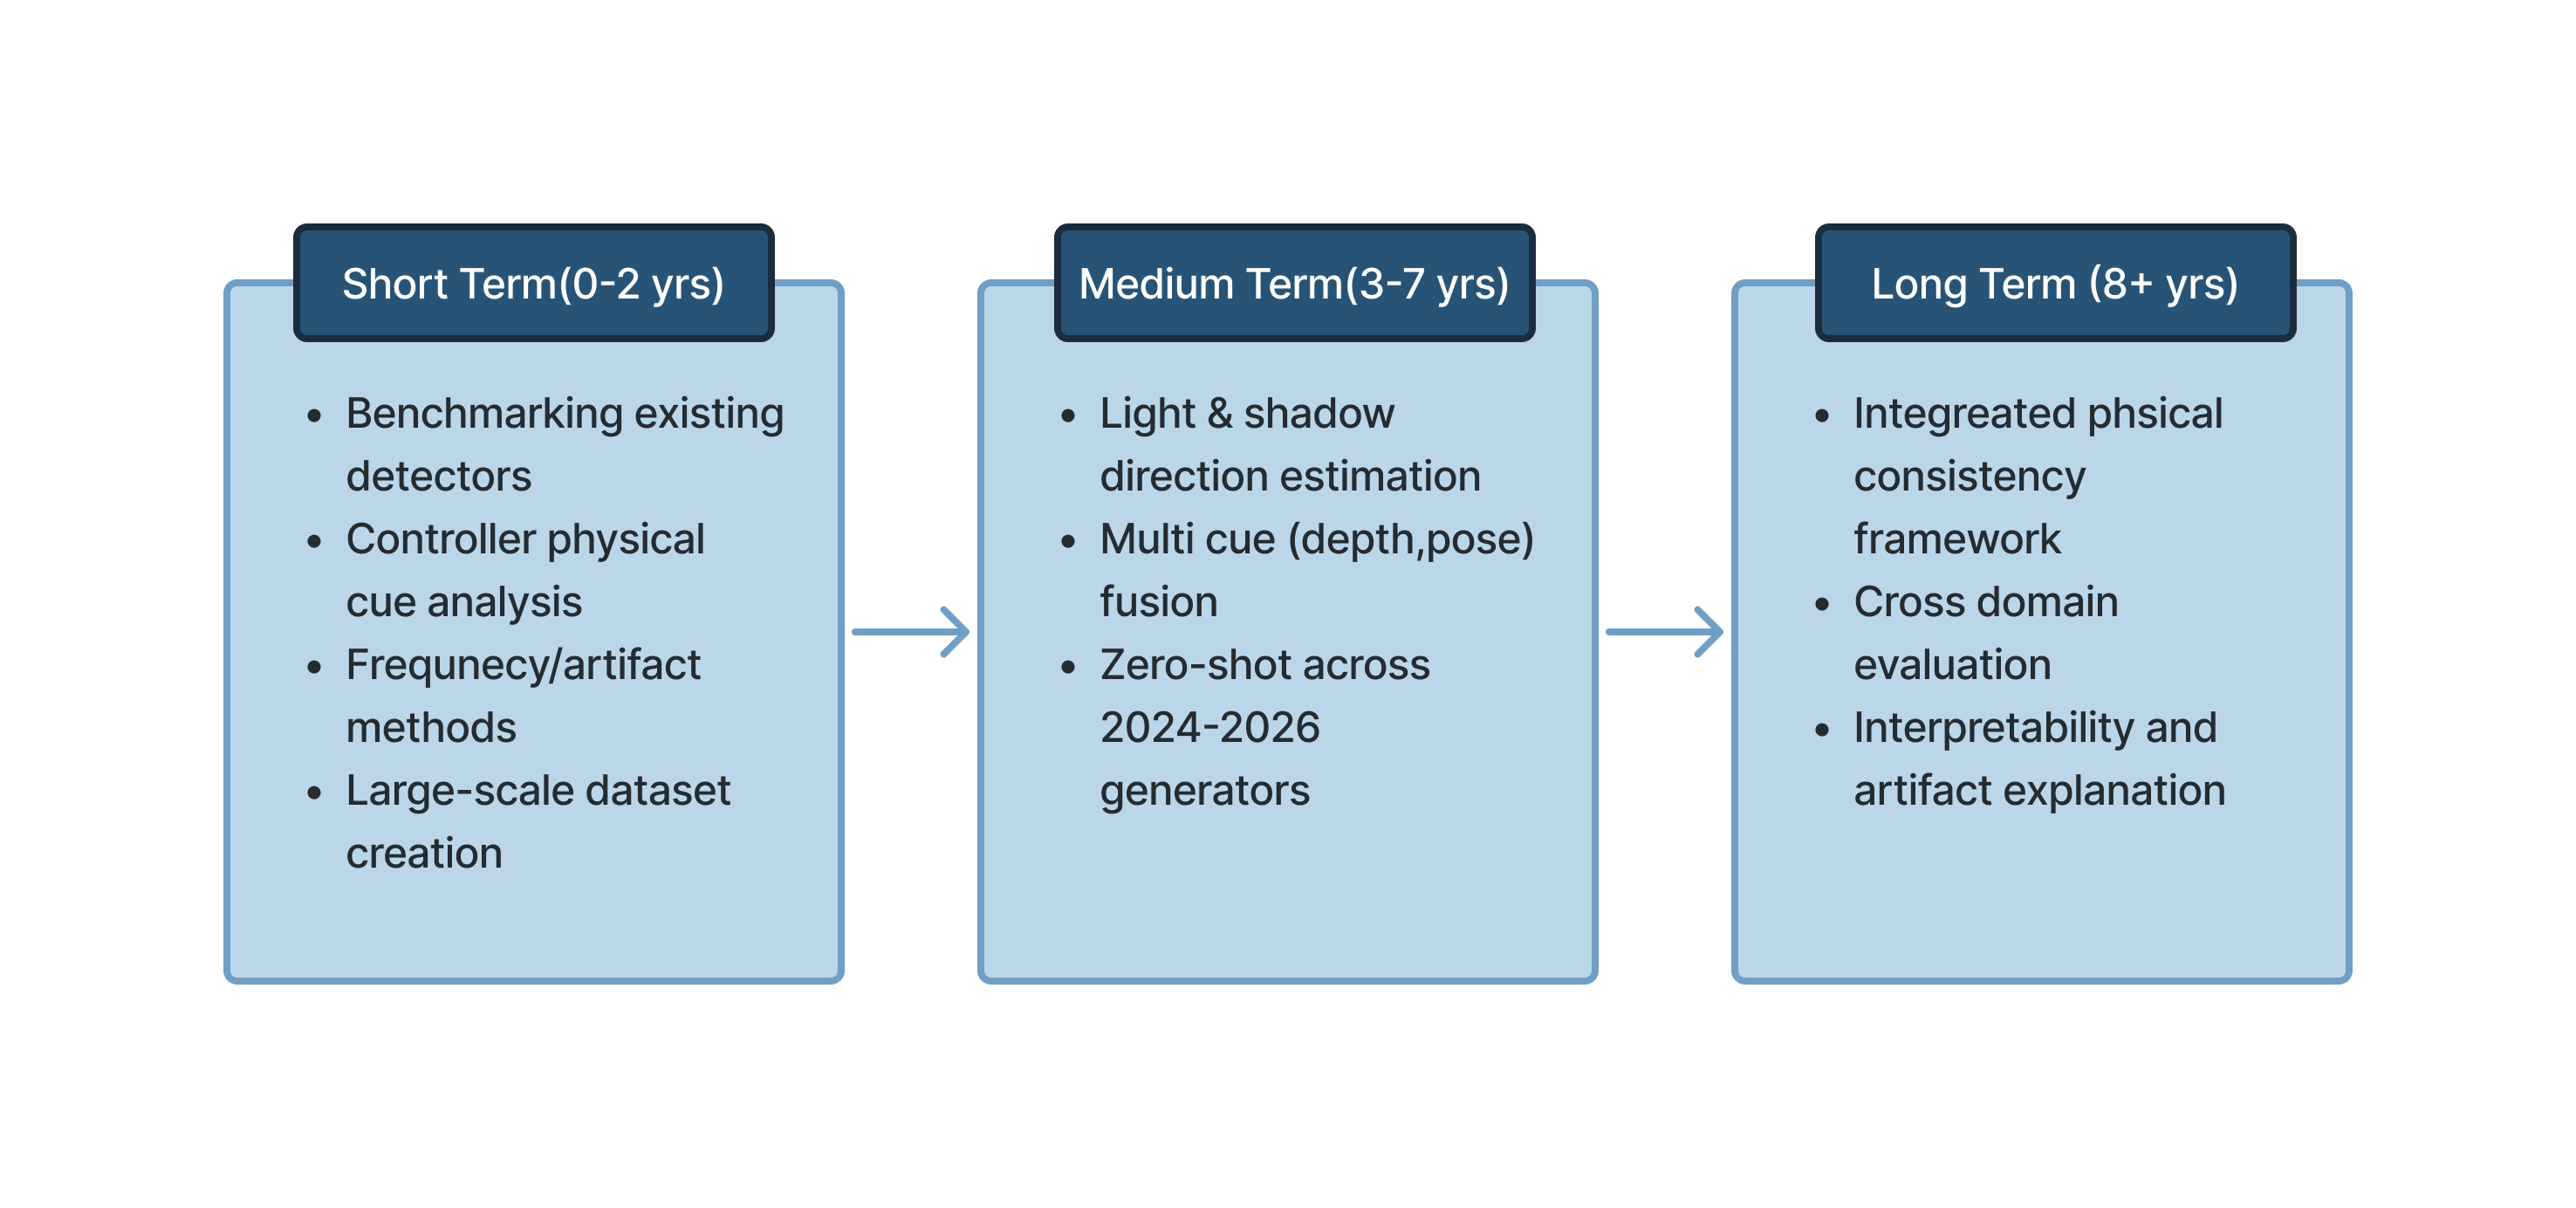
\includegraphics[width=\linewidth]{Pictures/Figure 6.png}
\caption{\textbf{Phased future-research roadmap.} Short-term items focus on benchmarking and single-cue analysis; medium-term items require multi-cue fusion across domains; long-term items integrate these into a comprehensive physical consistency framework.}
\label{fig:roadmap}
\end{figure}
\FloatBarrier

\section{Conclusion}
This systematic review examined 61 primary studies on AI-generated image and deepfake detection, organized into nine thematic clusters. The synthesis provides converging evidence that (a) statistical and frequency artifact learners consistently fail under domain shift, (b) pretrained semantic features improve generalization but forfeit interpretability, and (c) physically grounded, multi-cue architectures modeling lighting, shadow, geometry, depth, and anatomical plausibility are both theoretically robust and empirically under-explored. This gap identifies a critical future research direction: the development of cross-generator, physics-aware forgery detection frameworks capable of robust, interpretable performance in rapidly evolving generative ecosystems.

\backmatter

\section*{Declarations}

\begin{itemize}
\item \textbf{Funding:} No external funding was received for this review.
\item \textbf{Conflict of interest/Competing interests:} The authors declare no competing interests.
\item \textbf{Availability of data and materials:} The structured data-extraction spreadsheet (title, author, method, summary, and limitation for all 72 compiled and 61 included records) underlying this review is maintained by the authors and available upon request.
\item \textbf{Registration and Protocol:} This review was not registered in an external protocol registry. No prior protocol was prepared; deviations from a pre-specified plan are therefore not applicable.
\end{itemize}

\bibliography{sn-bibliography}

\end{document}